% status: 0
% chapter: TBD

\title{Apache CloudStack}


\author{Rashmi Ray}
\affiliation{%
  \institution{Indiana University}
  \streetaddress{}
  \city{Bloomington} 
  \state{IN} 
  \postcode{47408}
}
\email{rashray@iu.edu}

\author{Gregor von Laszewski}
\affiliation{%
  \institution{Indiana University}
  \streetaddress{Smith Research Center}
  \city{Bloomington} 
  \state{IN} 
  \postcode{47408}
  \country{USA}}
\email{laszewski@gmail.com}


% The default list of authors is too long for headers}
\renewcommand{\shortauthors}{G. v. Laszewski}


\begin{abstract}

  In this ever-evolving age of cloud computing, it is important for
  organizations to adopt the right cloud orchestration tool to promote
  the rapid growth of their infrastructure. Ease of maintainance, 
  robust research-base for future growth
  also facilitates the process. CloudStack can be the solution to 
  the problem. Apache CloudStack is a top level project from Apache, so it
  indeed has a support of a solid team of researchers.

\end{abstract}

\keywords{hid-sp18-417, CloudStack, apache, cloud architecture, cloud
  technology, i516}

\maketitle

\section{Introduction}

``Apache CloudStack is open source software designed to deploy and
manage large networks of virtual machines, as a highly available,
highly scalable Infrastructure as a Service (IaaS) cloud computing
platform. CloudStack is used by a number of service providers to offer
public cloud services, and by many companies to provide an on-premises
(private) cloud offering, or as part of a hybrid cloud
solution.''~\cite{hid-sp18-417-www-cloudstack-intro}. It is a Java based project.


\section{History}

The CloudStack was originally developed by cloud.com formerly know as
VMOs.  The project started in 2008 and was released under GNU general
public license.  In 2010, Microsoft partnered with cloud.com to 
facilitate support of microsoft server intergration. 
In Jul 2011 Citrix purchased the software and
released it again. In 2012 Citrix renewed CloudStack licensed under
the Apache and later donated the project to Apache.  Since then The
tool has graduated from Apache incubator and released in Mar 2013.


\section{Key Features}

\paragraph{Hypervisor Support:} A hypervisor or Virtual Machine
Monitor is a software or firmware that creates and runs virtual
machines. CloudStack currently supports most of the major hypervisors.
CloudStack enables a single cloud to constitute of multiple types of
hypervisor implementations. This is considered a key advantage when
implementing CloudStack on an existing infrastructure to enable
maximum use of the existing resources. 

\paragraph{Massively Scalable:}
``CloudStack can manage tens of thousands of physical servers installed
in geographically distributed datacenters. The management server
scales near-linearly eliminating the need for cluster-level management
servers. Maintenance or other outages of the management server can
occur without affecting the virtual machines running in the cloud''~\cite{hid-sp18-417-www-cloudstack-scalability}.

\paragraph{High Availability:} CloudStack provides features to
increase availability. It enables the management server deployed
across multiple nodes, this increasing availability through load
balancing. MYSQL can be configured simulate a replication that can
serve as a fallback in case of data loss. The tool also provides a
{\bf robust rest API} for operation and management of the cloud. The
API can be used with a CloudStack system as the underlying server.
The software also provides Amazon Web Services compatible
API. ``CloudStack provides an EC2 API translation layer to permit the
common EC2 tools to be used in the use of a CloudStack
cloud.''~\cite{hid-sp18-417-www-cloudstack-aws} The tool also eases
configuration management, Hypervisor agnostic, user management,
snapshot management and networking resource optimization.

\paragraph{GUI:} It might not be a prominent advantage for the cloud
computing community as it mostly prefers to carryout instruction in
the console, but for occasional users it is an added benefit that
CloudStack provides an efficient customizable Graphical User
Interface. In all CloudStack provides a comprehensive package of
features that can enable an organization to deploy a full featured
cloud Infrastructure. ClaoudStack also offers CloudMonkey CLI 
tool to easy orchestration from console.

\section{Terminology}

It is important to be aware of certain terminology to get an idea on
how resources are organized in CloudStack. Grouping resources 
appropriately enhances availability and fault tolerance. Here is the 
list in descending order in terms of size:
\paragraph{Region:}	The largest available unit in CloudStack infrastructure is a 
region. In case of a large Cloud network its ideal to group it into 
several geographic regions. A region may consist of multiple datacenters
located in proximity. It can be managed by one or a cluster of management
servers. Data can be spanned across multiple regions so that in case of
failure of one region the services will still be available from other regions(s).
\paragraph{Zone:}	A zone typically consists of a datacenter. A zone can have its own LAN
network and supply line. 
\paragraph{Pod:}	A pod is typically a rack or cluster(s) of hosts. Hosts in a Pod are 
expected to be in same subnet. 
\paragraph{Cluster:} 	A cluster is a group of hosts that can be a pool of VMwares or KVM 
servers. ``The hosts in a cluster all have identical hardware, run the same 
hypervisor, are on the same subnet, and access the same shared primary storage.
Virtual machine instances (VMs) can be live-migrated from one host to another
within the same cluster, without interrupting service to the user''~/cite{hid-sp18-417-www-cloudstack-cluster}
\paragraph{Host:}	A host is a single node/machine that has hypervisor installed.
\paragraph{Storage:}	At least one Primary Storage is associated with a cluster or zone. The 
storage is available to each cluster in the zone and store a virtual copy of 
each VMs to be used in case of failure. CloudStack also offers a secondary storage
option for ISO images and snapshots.
Figure~\ref{F:cloudstack-resource-group} depicts how resource can 
be grouped in a CloudStack deployment.
\begin{figure}[htb]
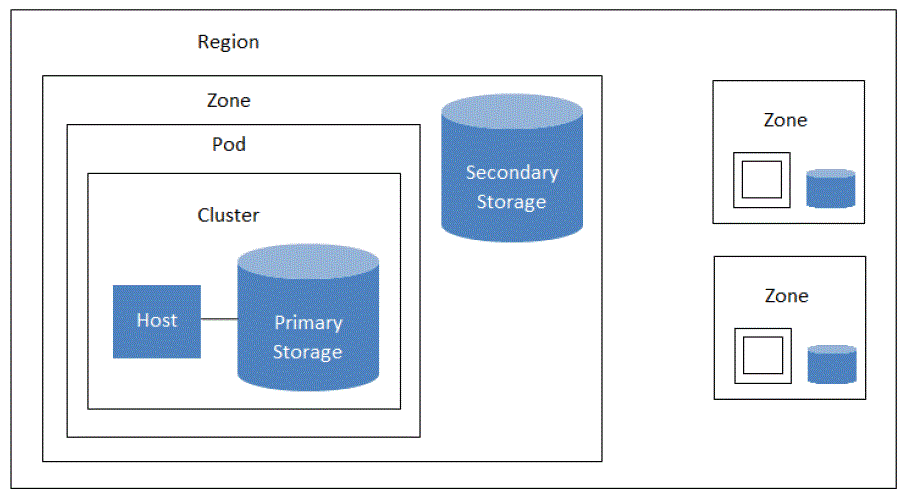
\includegraphics[width=\textwidth]{../images/hid-sp18-417-cloudstack.png}
\caption{CloudStack Resource Organization~\cite{hid-sp18-417-cloudstack-resource-grouping}}
\label{F:cloudstack-resource-group}
\end{figure}

\section{Deployment Architecture}

To use CloudStack, several deployment architectures can be adopted
depending on the cloud requirements of an organization. The strength
of the deployment can range from a single machine to thousands of
nodes spread across the globe in several data centers several
networking technologies.

\paragraph {A CloudStack deployment} primarily consists of a management server and
set of resources [IP addresses, VLANs, storage systems] to constitute
the cloud.  For simplest form of deployment, only one single machine
can be used to serve both as the management server and hypervisor
host. The same system can be scaled to feed increased demand to spread
across multiple management servers to support larger userbase and
facilitate better load balancing. ``The management server typically runs
on a dedicated machine or as a virtual machine. It controls allocation
of virtual machines to hosts and assigns storage and IP addresses to
the virtual machine instances. The Management Server runs in an Apache
Tomcat container and requires a MySQL database for
persistence.''~\cite{hid-sp18-417-www-cloudstack-management-server} 
The management server as the name suggests provides the single point 
Management controlling the configurations, snapshots, resources monitoring, 
API, Web Interface etc. 

\paragraph {pluggable model} CloudStack supports a pluggable model. This model enables 
different features to fit in as different components. ``Customers may 
choose SDN support from Nicira, Midokura or Big Switch Networks and choose 
load balancing using NetScaler or F5. For object storage, CloudStack offers a
choice of products from Basho, Caringo, Cloudian or EMC's Atmos. Users also 
may choose OpenStack's Swift component.’’ ~\cite{hid-sp18-417-www-cloudstack-model }
This model provides flexibility for the organizations to scale their infrastructure
using latest technology as well as reusing the existing resources.

\section{Installation}

Before the CloudStack installation it is important to decide on the resources,
deployment architecture-based on resources, hypervisors, network and storage 
configurations. The management server needs Cent OS or ubuntu operating system
with 64bit x86 processor. The server needs a minimum of 4 GB RAM and 250 GB
hard disk space. 

\paragraph () Each of the host must have hypervisor installed that is Hardware
Virtual Machine[HVM] supported. A host optimally needs 64bit x86 processor, 4 GB
RAM, 36 GB hard disk. Each of the machines needs at least 1 Network Interface Card 
to connect to the cloud network.  After the OS installation vh-util need to be installed 
in case Xen server. Now is time to install and configure the very first management 
server following by setting up the mysql DB. Once the DB is setup it is important to 
setup Primary and Secondary storage for high availability. Finally, the system virtual 
machine template needs to be prepared for the secondary storage. Please note
 that additional management servers can be added if required.

\paragraph {Package Repository}: ``CloudStack is only distributed from source from the official
mirrors. However, members of the CloudStack community may build convenience binaries 
so that users can install Apache CloudStack without needing to build from source.''~\cite{hid-sp18-417-www-cloudstack-package-repo}


\section{Security}
CloidStack has a dedicated security team to identify possible vulnerabilities and address to breach reports. 

\section{Conclusion}

CloudStack provides a comprehensive package or unique features and flexibility for the 
organization to develop a robust cloud architecture. The platform being an open source projec
from Apache foundation, it provides a regular stable updates and releases that enables it to 
stay in put with the latest in the industry. There is a strong developer community support
being CloudStack. CouldStack community normally releases a long term release every two years.

\paragraph {CustomerBase:} There can be short term releases for bug fixes or security patches.
The most recent source release of CloudStack is 4.11.0.0. Even if it provides a comparatively smoother deployment,
it still involves a time-consuming process with several steps. For this purpose, some community 
members provide package repositories for easier installation and deployment. 
Regular events are being conducted all over the world to promote team collaborations and 
contributions. Datapipe is one of the major user of CloudStack. The major users of CloudStack
includes: Apple , Citrix Systems, Dell, Disney, Hitachi , Juniper Networks, PPTV, SAP, 
WebMD etc. 


\begin{acks}

  The author would like to thank Dr.~Gregor~von~Laszewski for his
  support and suggestions to write this paper.

\end{acks}

\bibliographystyle{ACM-Reference-Format}
\bibliography{report} 
